\documentclass{sbrt2017port}

\usepackage{cite}
\usepackage[cmex10]{amsmath}
%\usepackage[pdftex]{graphicx}
\usepackage{url}
\usepackage[caption=false,font=normalsize,labelfont=sf,textfont=sf]{subfig}
\graphicspath{{img/}}
\DeclareGraphicsExtensions{.pdf,.jpeg,.png}


\begin{document}
\title{Detecção de pessoas em um ambiente industrial utilizando imagens de profundidade e classificadores profundos}

\author{Eduardo Henrique Arnold e Danilo Silva\thanks{Eduardo Henrique Arnold e Danilo Silva. Departamento de Engenharia Elétrica, Universidade Federal de Santa Catarina, Florianópolis, Brasil, E-mails: eduardoarnoldh@gmail.com e danilo@eel.ufsc.br. } }

\maketitle

\markboth{XXXV SIMPÓSIO BRASILEIRO DE TELECOMUNICAÇÕES E PROCESSAMENTO DE SINAIS - SBrT2017, 3-6 DE SETEMBRO DE 2017, SÃO PEDRO, SP} {XXXV SIMPÓSIO BRASILEIRO DE TELECOMUNICAÇÕES E PROCESSAMENTO DE SINAIS - SBrT2017, 3-6 DE SETEMBRO DE 2017, SÃO PEDRO, SP}

\begin{resumo}
asd
\end{resumo}

\begin{chave}
Chaves
\end{chave}

\begin{abstract}
This paper describes the development of an industrial safety system that requires automatic human detection. Two solutions based on top-view depth images are presented. The first one is based on traditional learning techniques using feature extraction and a Support Vector Machine classifier. The second solution uses deep learning methods for classification. The performance analysis of both solutions revealed that the deep learning methods outperform traditional learning techniques on this task, at the cost of requiring a larger training set and increased computational complexity.
\end{abstract}

\begin{keywords}
  Human detection, depth images, deep learning, SVM, machine learning, computer vision.
\end{keywords}

\section{Introduction}
  In any industrial facility workers safety must be a priority. There are certain areas that offer higher risk and thus should not be occupied during regular operation. An example is given by a home appliance factory that uses an overhead crane to shift iron molds towards plastic extruding machines. These molds can be very heavy, offering risks to anyone working underneath the moving crane.

  In this context it is helpful to have an automatic safety system that detects humans on the path of the moving machine and causes it to halt in the event it finds a person. A video based solution would be ideal in this case, especially considering that the factory environment is crowded with machines, molds and workers. Since the crane will be moving, the camera should be placed underneath it,  facing the factory floor. This poses a challenge as background subtraction methods cannot be applied, requiring a more sophisticated detection algorithm.

  Another challenge is that workers clothes are not regular in color, and they do not always wear helmets, in which case only color images could not give enough information for detection. To overcome this, \cite{rauter} uses a stereo camera that delivers depth image frames of objects, providing more reliable shape information and higher invariance to luminosity. The image is then used to locate human candidates, followed by a hand-engineered feature extraction and then classification using a Support Vector Machine (SVM). However, this approach may not provide a good solution given the differences in the environment since it assumes a clean standarized ambient, as opposed to a crowded industrial facility.

  Recently the increase of computational power, especially in GPUs, the availability of large image datasets and improvements upon existing training methods \cite{nair2010relu}, along with dense network structures \cite{NIPS2013_5207} made the fast development and usage of deep learning methods in most diverse domains, breaking previous state-of-the-art results \cite{hintonCONVNET}. The main advantage of deep learning methods is that it shifts the focus from feature-engineering to a data-driven approach, in the sense that the network structure itself will learn how to best represent the input data, as long as it has enough samples to learn from. Motivated by this, another approach to the human detection could be developed by using top-view depth images and deep classifiers.

  This paper makes a comparison between two approaches to the human detection system, illustrated in Figure \ref{fig:system-diagram}. Both uses computer vision techniques to detect candidates in the image, described in Section \ref{sec:candidates}. The first solution, based in \cite{rauter}, is presented in Section \ref{sec:classical}, while the latter, using deep classifiers, is described in Section \ref{sec:deep}. Quantitative evaluation of both methods and their variations is shown in Section \ref{sec:results}. Finally, conclusions and future work are presented in Section \ref{sec:conclusion}.

  \begin{figure*}[!t]
  \centering
  \includegraphics[width=\linewidth]{system-diagram.png}
  \caption{Human detection system diagram.}
  \label{fig:system-diagram}
  \end{figure*}

\section{Candidates detection}
\label{sec:candidates}

    In a traditional object detection approach \cite{traditional-objdetect} the first step is to localize candidates, which are then validated using a feature-extractor followed by a classifier. In the case of a color image, a sliding window method with varying size could be used to obtain such candidates.

    However, when using depth images from a top-view scene, \cite{rauter} suggests a more efficient algorithm that assumes that humans will be among the highest objects in the scene. Although this hypothesis cannot always be guaranteed, it reduces the amount of candidates significantly when compared to the sliding window method and so is used in this work and described next.

    First, a local maxima operation is performed. It divides the image in a grid of specified-sized blocks and for each block returns the pixel with highest intensity, representing the tallest point in that block. Next, for each local maxima a squared window representing the candidate should be obtained. Its size is calculated as
    \begin{equation}
      s_w = \frac{f}{d} \cdot s_r
    \end{equation}
    where $f$ is the camera focal distance, $d$ the distance between the camera and the object and $s_r$ the mean head size. The window of size $s_w$ pixels is centered around the respective local maximum pixel.

    The final step is to centralize the window over the candidate using an iterative \textit{mean shift} algorithm. Simply put, this algorithm displaces the window to the centroid of the pixels inside it, so high valued pixels will tend to be in the center of the candidate.

    The output of this step is a list of squared windows representing candidates in the image. A relevant aspect to consider is the size of the blocks for the local maxima search. When using large blocks the probability of having a tall object, such as a machine, in the same block of a person is high, so the system would fail to detect a person. In contrast, if the block is too small, it is guaranteed that all humans will be detected, but this comes at the expense of complexity and time performance, since all candidates will need further analysis.

\section{Classical computer vision solution}
\label{sec:classical}

    Following the candidates detection a validation phase should take place to discard non-human detections. A classical computer vision approach \cite{rauter} uses hand-engineered features extracted from the candidates to feed a binary SVM classifier, which output a class: ``human'' or ``not human''. A regular block grid proposed in \cite{rauter} is used. In order to increase rotation invariance, we also propose a concentric rings descriptor (see Figure \ref{fig:descriptors}). Both are described next, followed by a more detailed description of the classification and training process.

    \begin{figure}
    \centering
    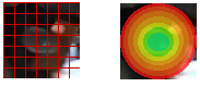
\includegraphics[width=0.9\linewidth]{tradicional/descritores}
    \caption{Regular block grid (left) and concentric rings descriptors (right).}
    \label{fig:descriptors}
    \end{figure}

    \subsection{Regular block grid feature extractor}
      This descriptor divides the candidate window into 7x7 blocks, as illustrated in Figure \ref{fig:descriptors}. The mean value of pixels belonging to each block is calculated, generating a 7x7 matrix of mean pixel intensities. Next, the mean value of the central block is subtracted from the matrix. Finally, the resulting matrix histogram is calculated with 32 bins. The histogram vector, with 32 dimensions, is considered the feature vector, which sums up to 49 (number of blocks).

    \subsection{Concentric rings feature extractor}
       First the candidate window is divided in 18 annulus, or rings, with equal distance between the inner and outer radius and whose center coincides with the window center. Then for each ring the mean of the pixels that belong to it is calculated, resulting in a 18 dimensional vector of mean pixel intensity. Next, the mean value of the inner ring (lower radius equals zero) is subtracted from this vector. Following, we perform a discrete differentiation of this vector (subtraction between adjacent dimensions) to enunciate the differences in rings mean values, resulting in a 15-dimensional feature vector.

    \subsection{SVM classifier}
      We use a binary SVM classifier with Radial Basis Function (RBF) kernel \cite{rbfkernel} to validate the candidates. Recall that the kernel parameter $\sigma$ along with the SVM hyper-parameter $C$ control the trade-off between training performance and generalization on unseen data. Higher $C$ values penalize training set errors, while lower values offer a more general performance on the test set, conversely, the $\sigma$ parameter penalizes in the inverse manner.

      To choose the appropriate values of the hyper-parameters $C$ and $\sigma$ we use a 5 fold cross-validation process, scoring the \textit{precision} metric \cite{evaluationMetrics}. Then a complete training using the entire training dataset, composed by 9894 negative samples and 1222 positive samples is performed. The dataset was generated from video samples collected at the factory during a experiment to test camera positions (placed at a height of 6m), each sample of the dataset is a window cut from a depth frame. These cuts are obtained with the candidate selection procedure presented in Section \ref{sec:candidates} and are manually labeled as positive (human) or negative (not human).

      The SVM classifier was implemented in Python using the Scikit-learn \cite{scikit-learn} toolkit.


\section{Deep learning based solution}
\label{sec:deep}

    Neural networks can be used to perform robust classification with complexity varying according to the network structure and depth. We use and evaluate two deep structures: multilayer perceptron (MLP) and convolutional neural networks (CNN). In our solution for both approaches, the candidate is resized to a 60x60 window and directly fed to the classifier, without any feature-extraction process. We can consider that the model itself will encode a feature set in the first layers of the network, with the final layer doing the classification process and outputing a single probability of that candidate being a human. The diagram would be the same as presented in Figure \ref{fig:system-diagram} without the feature extraction block and with a real valued output probability.

    \subsection{Multilayer perceptron}toolkit
        The MLP structure is composed by units organized in layers. Every unit in a single layer is connected to every unit on the following layer. Each unit calculates its output by summing of its inputs, weigthed by the connections parameters, and then applying an activation function $\phi(x)$. Each output is forward propagated through the network from the input layers, through the hidden layers until the output layer.

        We use a structure with 3600 input units (60x60 pixels), 512 and 256 units in the hidden layers and a single unit in the output layer, as seen in Figure \ref{fig:diag-mlp}. The hidden layers, shown in yellow, use the RELU \cite{nair2010relu} activation function to avoid the vanishing gradient problem. The single output unit uses a sigmoid activation function to reproduce a probabilistic output.

        \begin{figure}
        \centering
        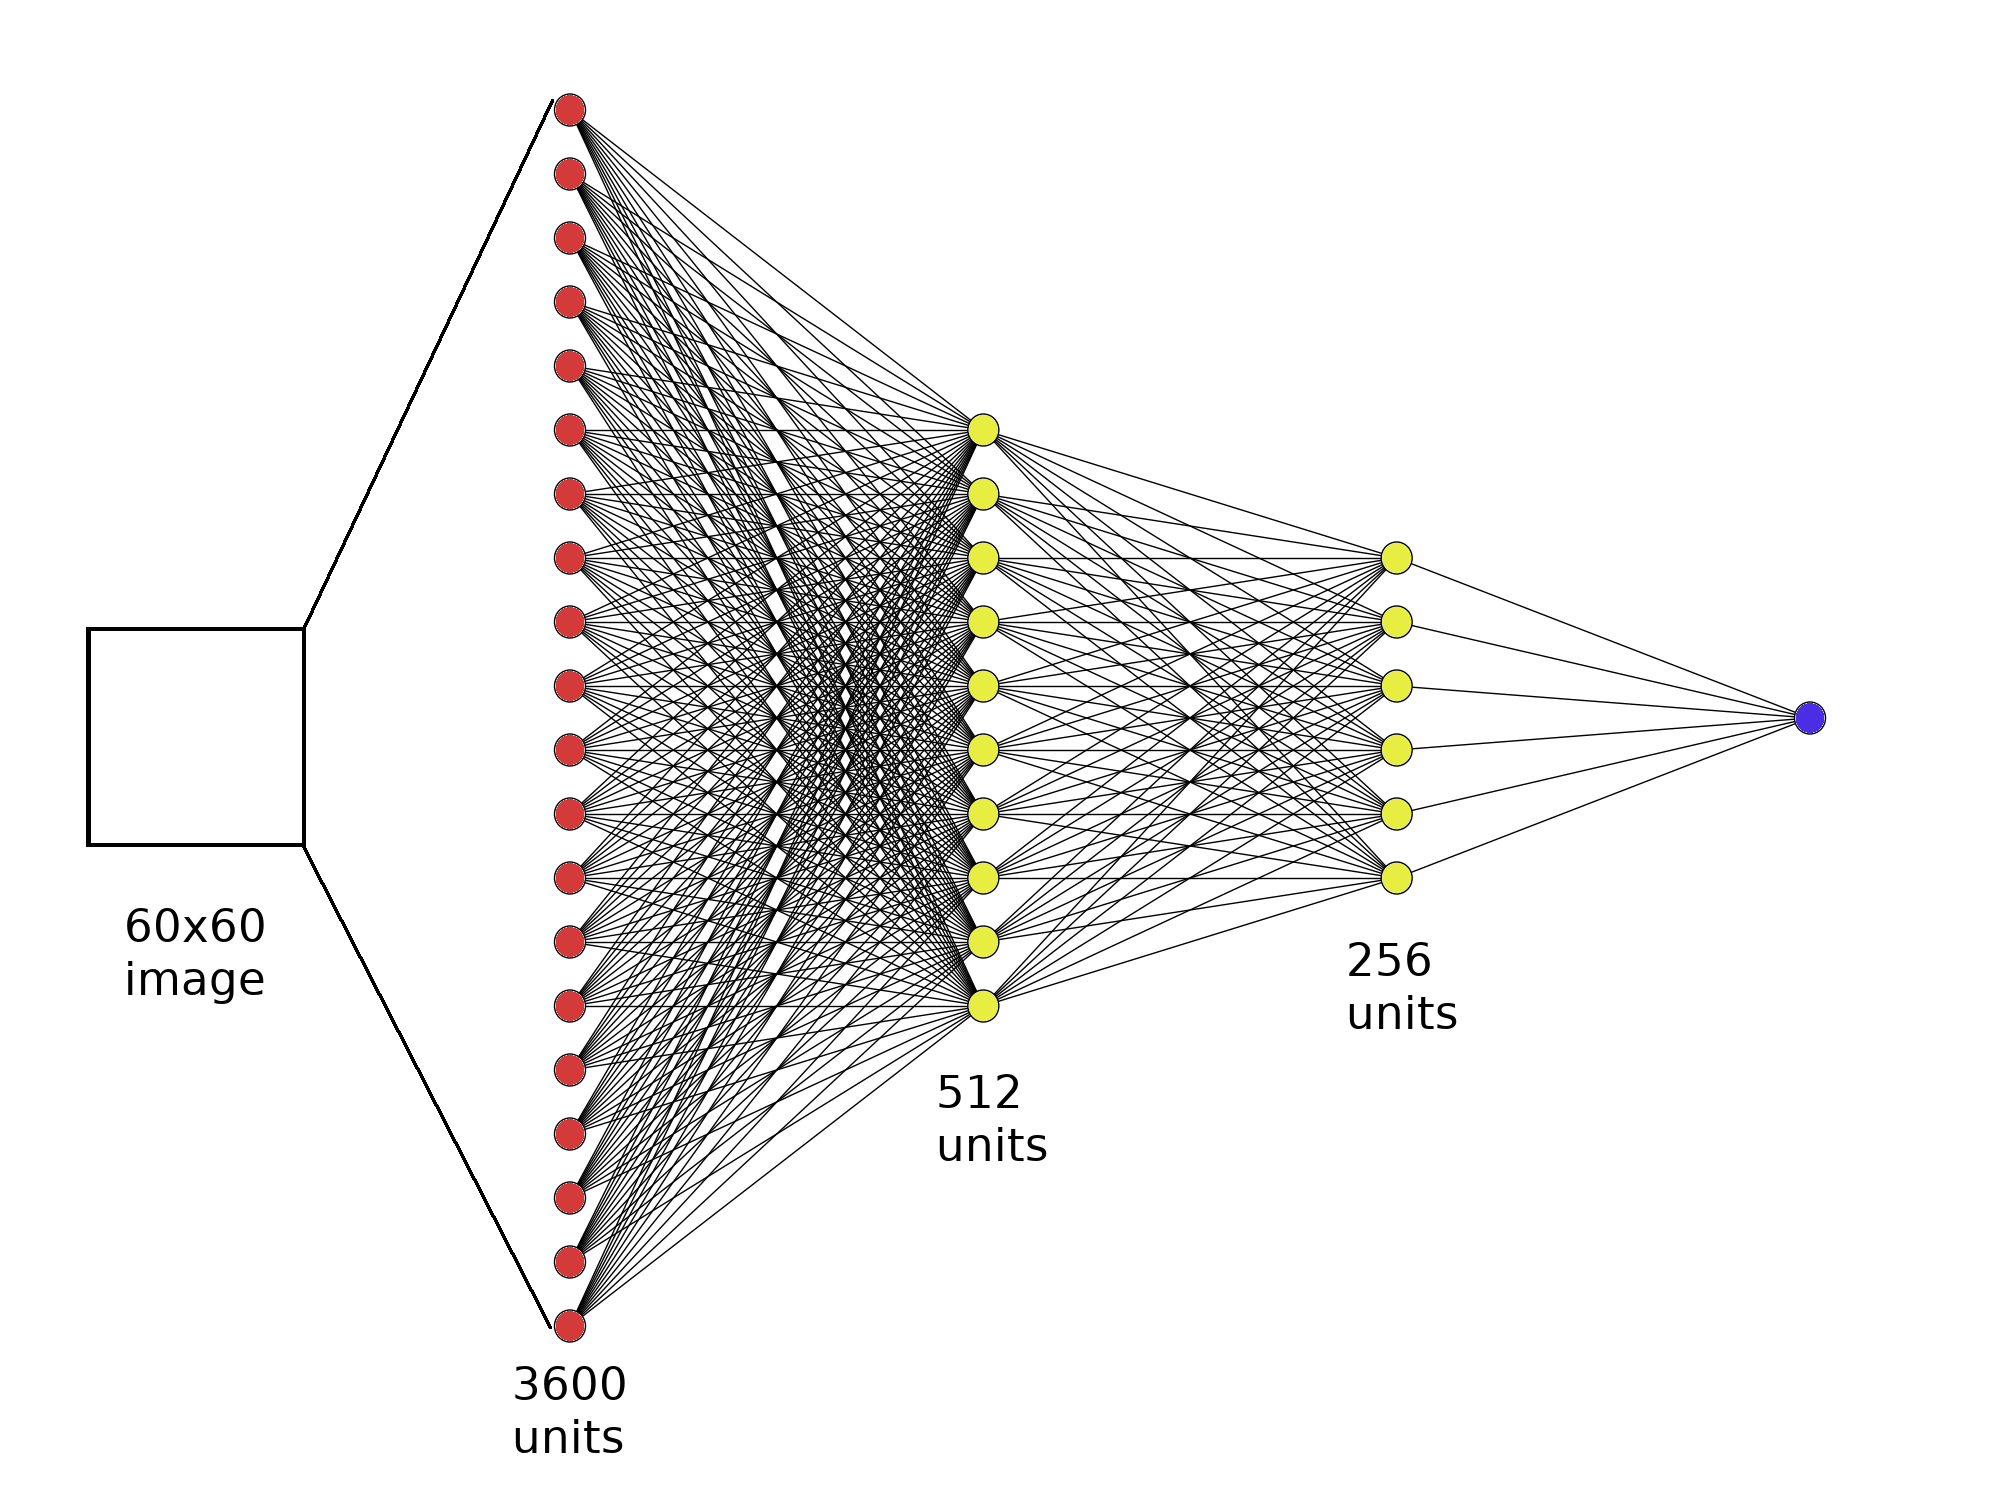
\includegraphics[width=0.8\linewidth]{diagram/diag-mlp.png}
        \caption{MLP network structure.}
        \label{fig:diag-mlp}
        \end{figure}

    \subsection{Convolutional neural network}
         In images there are strong local correlation of pixels, so it is not necessary that every unit in each layer is connected to every unit in the following layer, but just to a few local neighbours. This local connectivity is achieved through the convolution of a given layer with a bank of filters. In this sense, convolutional neural networks are a derivation of MLP and, in general, give a better model for images by reducing the number of parameters thus helping to generalize.

        Our CNN structure, depicted in Figure \ref{fig:diag-cnn}, is composed by a 3x3 convolution layer with 16 feature maps (filters), followed by a 3x3 max pooling layer, then flattening resulting in 5776 (16x19x19) units followed by a 128-units dense layer to perform classification, and finally by a single output unit that gives a probabilistic output. Again, the hidden layers use RELU activation and the output unit uses sigmoid activation.

        \begin{figure}
        \centering
        \includegraphics[width=0.9\linewidth]{diagram/diag-cnn.png}
        \caption{CNN network structure.}
        \label{fig:diag-cnn}
        \end{figure}

    \subsection{Implementation}
        The training process consists of minimizing an objective function, in this case, the binary cross-entropy function \cite{DLbook}, also known as logloss. Its use is justified by the probabilistic nature of the output layer. The optimization method used is a variation of Batch Stochastic Gradient Descent (B-SGD) called Adam \cite{kingma2014adam}, which uses an adaptive learning rate based on momentum considerations (gradient based) for each parameter.

        Since deep models require a larger training set, we extended the SVM training set to 16898 samples, from which 14966 are negative. A challenge faced during the training phase was the impossibility of getting a coherent model due to the unbalanced distribution of the dataset: more than 88\% of the samples belonged to the negative class, so the model would classify all the samples as negative and still get a relative high accuracy. To overcome this, we artificially balanced our training set by replicating positive samples until their frequency was the same as the negative class.

        The computer vision task, candidate extraction, resizing, was done in C++ with the OpenCV library. The deep classifier was implemented using Keras \cite{keras} on top of Theano \cite{theano}, allowing GPU acceleration and enabling a fast training process (an epoch per minute).


\section{Results}
\label{sec:results}

    The evaluation uses Receiver Operating Characteristic (ROC) curves \cite{evaluationMetrics} to compare between solutions and parameters. These curves are generated from the probabilistic output of the classifiers used. In the case of SVM which under original formulations is a non-probabilistic classifier, we use a logistic regression formulation \cite{svmProbabilisticOutput} to enable a probabilistic output. The advantage of using such a probabilistic output classifier is the possibility of adjusting the true-positive vs false-positive tradeoff even after training, by choosing the probability threshold above which the sample is considered to be positive.

    To evaluate the solutions proposed on Sections \ref{sec:classical} and \ref{sec:deep}, with their variations, we firstly consider the candidates already extracted from a video sequence, which will be called the test set, thus evaluating only the descriptor and classifier. Figure \ref{fig:result-classifiers} shows the performance of the classifiers under the test set and a Area Under Curve (AUC) score \cite{evaluationMetrics} (measured up to 10\% of false-positive rate). We can clearly see that deep based classifiers outperform the traditional hand-engineered feature extraction based approach. Although both MLP and CNN perform similarly, one of them can be chosen depending upon the desired region of operation (higher true-positive rate or lower false-positive rate).

    \begin{figure*}[!t]
    \centering
    \subfloat[]{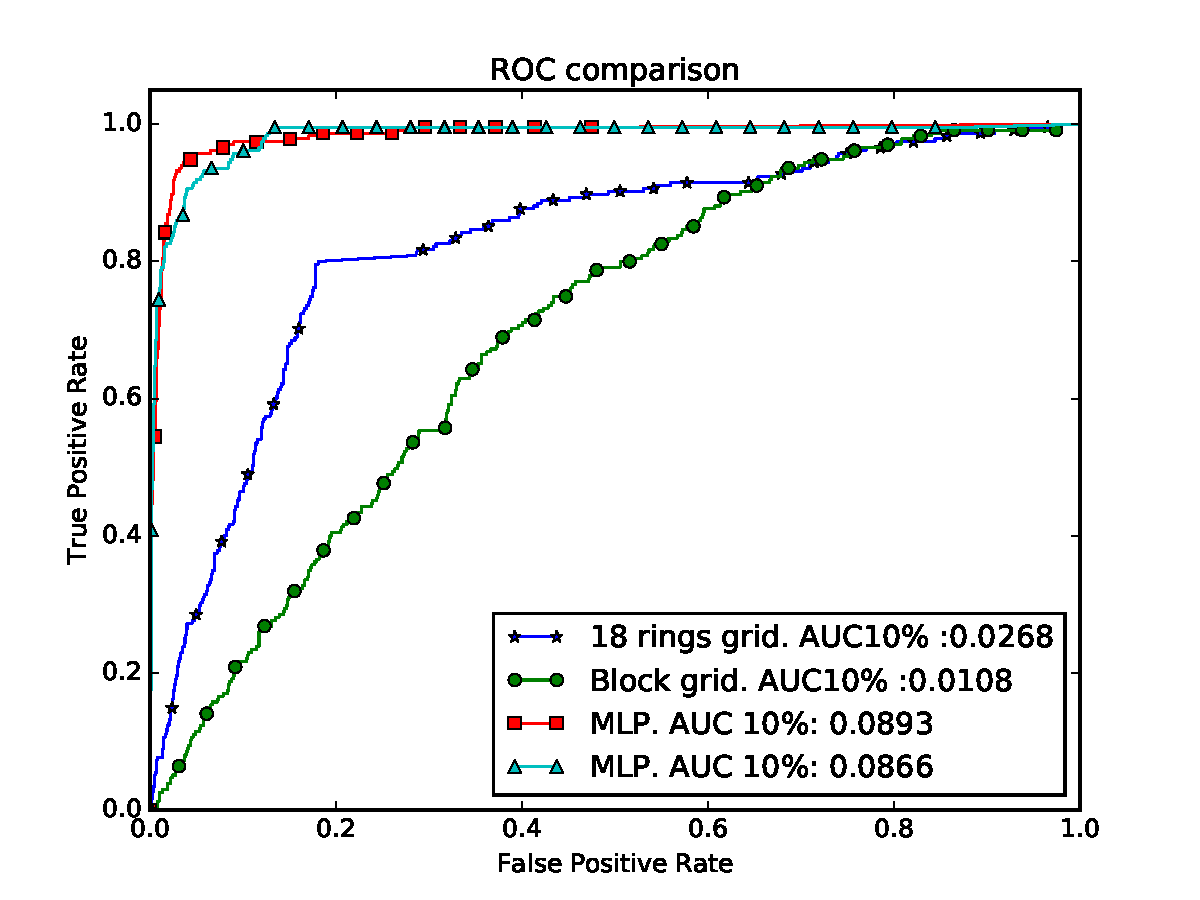
\includegraphics[width=0.45\linewidth]{results/ROC_all.pdf}}%
    \label{fig:result-classifiers-all}
    \hfil
    \subfloat[10 \% interest zone]{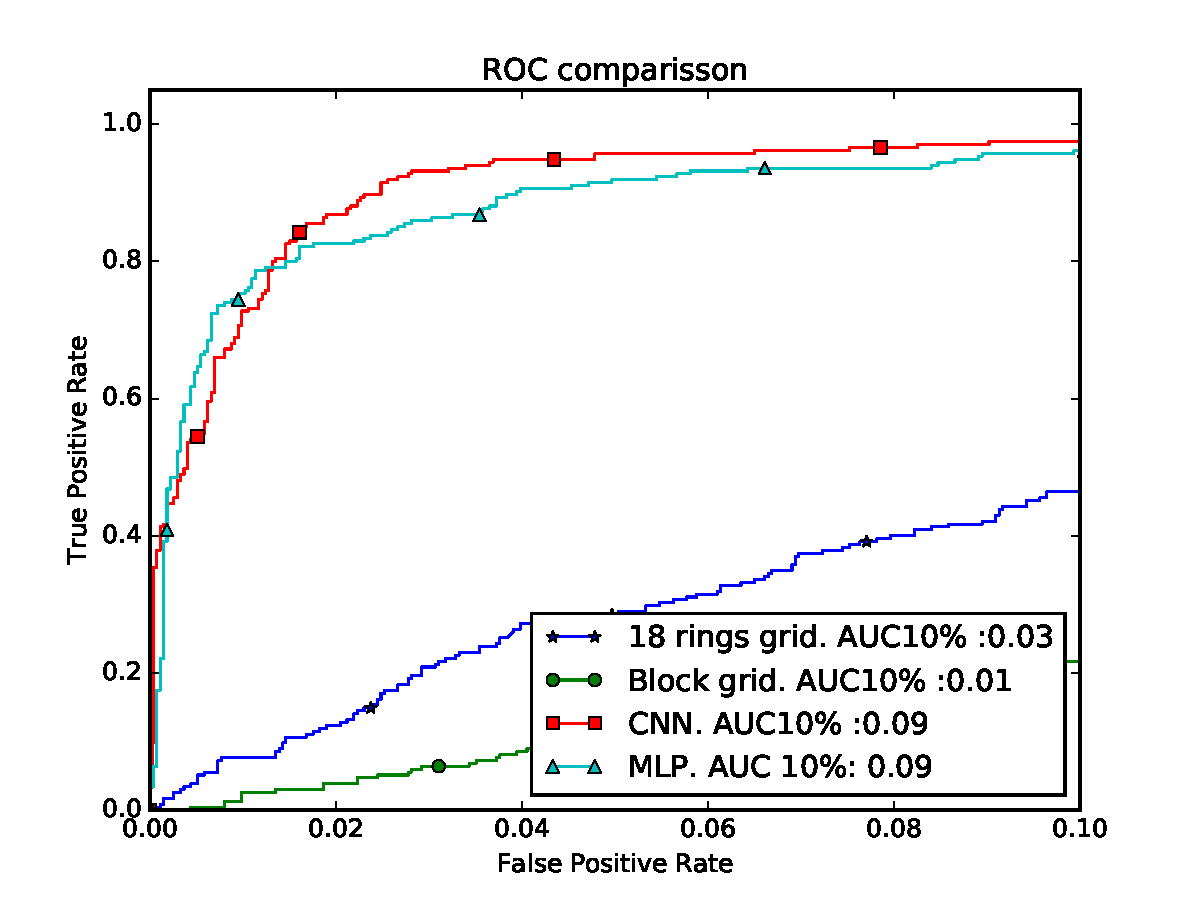
\includegraphics[width=0.45\linewidth]{results/ROC_all_zoom.pdf}}%
    \label{fig:result-classifiers-all-zoom}
    \caption{Classifiers performance.}
    \label{fig:result-classifiers}
    \end{figure*}

    In a second phase we consider the overall system performance, including the candidate extraction step. It is important to note that the performance observed in Figure \ref{fig:result-classifiers} is an upper bound of the overall performance, since now there will be miss-detections from the candidate extraction step. Another consideration is that in this phase the test set is composed of entire frames, so the probability of the frame contain at least one head could be calculated using
    \begin{equation}
    P[y=1] = 1 - \prod_i^n (1-p_i)
    \end{equation}
    where $y$ is a random variable valued 1 if there are humans in the scene or 0 otherwise, $n$ is the number of candidates and $p_i$ is the classifier output of candidate $i$. Figure \ref{fig:result-system} shows the overall system performance using this formulation with the combinations of MLP and CNN classifiers with coarse and fine scales of candidate extraction windows.

    The results show that on a coarse scale detector, the MLP and CNN classifiers have similar performance, because the candidates that get extracted have similar outputs. However, on a fine scale detector, many more candidates are detected so there are more samples to explore the performances of the two classifiers, showing how the CNN model outperforms MLP.

    \begin{figure*}[!t]
    \centering
    \subfloat[]{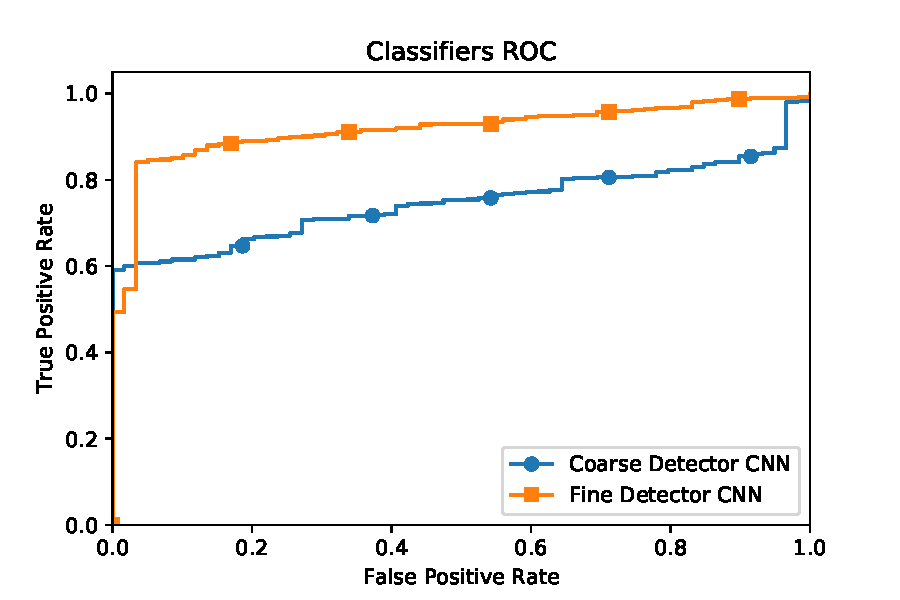
\includegraphics[width=0.45\linewidth]{results/ROC_system.pdf}}%
    \label{fig:result-system-all}
    \hfil
    \subfloat[10 \% interest zone, best results]{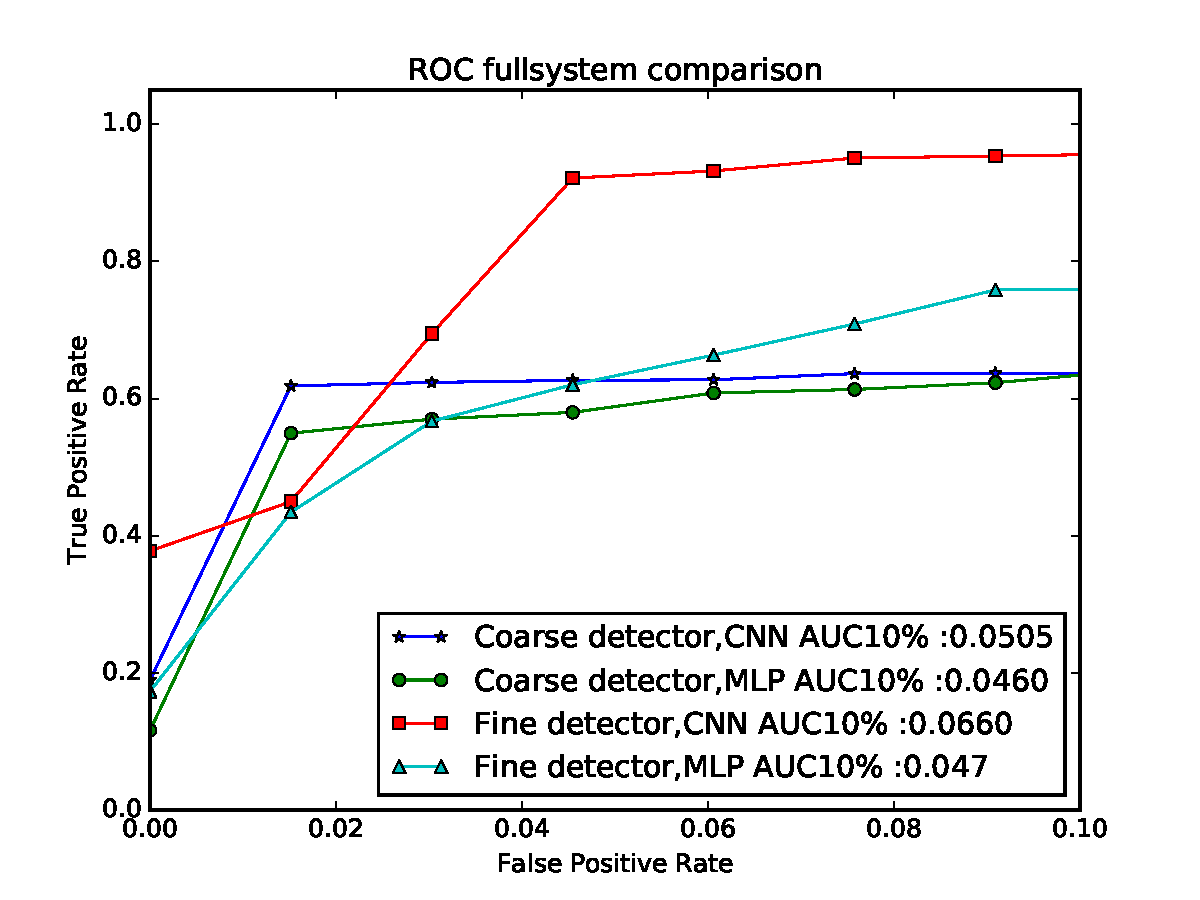
\includegraphics[width=0.45\linewidth]{results/ROC_system_zoom_best.pdf}}%
    \label{fig:result-system-all-zoom}
    \caption{Overall system performance.}
    \label{fig:result-system}
    \end{figure*}

\section{Conclusion}
\label{sec:conclusion}

    This paper investigates two solutions for the human detection problem, one based on traditional computer vision methods and another on deep learning techniques. The results presented in Section \ref{sec:results} show that the last method outperforms traditional hand-engineered feature extraction and classification, although they require a larger training set and have higher complexity, thus requiring more processing power. While deep learning techniques are widely regarded as useful for big datasets, we were still able to achieve good performance, even under a moderate-sized unbalanced dataset.

    One possible direction of future work is investigating a more general CNN structure. Instead of receiving just the candidate window, it would receive the whole depth frame as input and output the probability that frame contains a human. As we saw an improvement of the classification by letting the model choose the best representation of the data, we suspect that allowing the model to access the whole frame as opposed to only small windows possibly containing humans will improve the overall system performance.


\nocite{*}
\bibliographystyle{IEEEtran}
\bibliography{main}

\end{document}
